Per svolgere questo esperimento sono stati innanzitutto scelti dei riferimenti:
\begin{itemize}
	\item La distanza tra la vaschetta e l'asta $d=(57.50\pm0.05)\ cm$.
	\item L'altezza dell'asta dalla quale sono state effettuate le osservazioni $D_0=(42.35\pm0.05)\ cm$.
\end{itemize}
Dopodiché è stata misurata l'altezza della vaschetta, ottenendo il seguente risultato: $D=(11.85\pm0.05)\ cm$. Queste tre grandezze sono state misurate utilizzando la riga. Per ognuna di loro sono state effettuate tre misurazioni e, poiché la loro semidispersione è minore dell'errore strumentale, la loro incertezza corrisponde proprio a quest'ultimo. Con queste tre misure è stato possibile stabilire, utilizzando la carta millimetrata posta sul fondo della vaschetta, il punto $O=(19.50\pm0.05) cm$ (vedi Figura(3)). Come mostrato in Figura (3) è possibile calcolare facilmente una stima dell'angolo di incidenza $\theta_i$:

\begin{equation}
	\theta_i=\arctan(\frac{d}{D_0-D})=62.06^{\circ}
\end{equation}

Mentre l'incertezza associata, dalla Legge (17) e ponendo $\vec{x_0}=(d,D_0,D)$, sarà calcolata con la relazione:

\begin{align}
	\Delta\theta_i&=\left(\frac{D_0-D}{d^2+D_0^2-2DD_0+D^2}\right)\Delta d-\left(\frac{d}{D_0^2-2DD_0+D^2+d^2}\right)\Delta D_0 + \\
    &+\left(\frac{d}{D^2-2D_0D+D_0^2+d^2}\right)\Delta D= \\ &=0.02^{\circ}
\end{align}

Facendo riferimento alla Figura (3), per ottenere una stima del coefficiente angolare $(\tan(\theta_i-\tan(\theta_r)))$ della retta espressa dalla Legge (1), sono state effettuate osservazioni dell'immagine $O'$ a dieci altezze $h$ dell'acqua differenti. Le altezze sono state misurate utilizzando la riga. Per ognuna di esse sono state catturate cinque misurazioni del punto $O'$ e, poiché la loro semidispersione è minore dell'errore strumentale, si anticipa che la loro incertezza corrisponderà all'errore strumentale. Il loro valore assoluto sarà invece la media delle diverse misurazioni. È stato poi calcolato il valore di $x$ (vedi Sezione (2.1)) e la sua incertezza è quindi data dalla Legge (23).

\subsection{Prima altezza}
\begin{equation}
	h_1=(1.25\pm0.05)\ cm
\end{equation}

\begin{table}[H]
	\centering
	\begin{tabular}{|c|}
		\hline
		\textbf{O' $[cm]$} \\
		\hline
		$18.40\pm 0.05$ \\
		$18.30\pm 0.05$ \\
		$18.30\pm 0.05$ \\
		$18.30\pm 0.05$ \\
		$18.40\pm 0.05$ \\
		\hline
	\end{tabular}
	\caption{Punti $O'$ misurati per la prima ampiezza.}
	\label{tab:}
\end{table}

Il punto $O'$ è quindi:
\begin{equation}
	O_1'=(18.34\pm0.05)\ cm
\end{equation}
mentre il valore di $x$:
\begin{equation}
	x_1=(1.16\pm 0.10)\ cm
\end{equation}

\subsection{Seconda altezza}
\begin{equation}
	h_2=(1.65\pm0.05)\ cm
\end{equation}

\begin{table}[H]
	\centering
	\begin{tabular}{|c|}
		\hline
		\textbf{O' $[cm]$} \\
		\hline
		$17.60\pm 0.05$ \\
		$17.70\pm 0.05$ \\
		$17.60\pm 0.05$ \\
		$17.60\pm 0.05$ \\
		$17.70\pm 0.05$ \\
		\hline
	\end{tabular}
	\caption{Punti $O'$ misurati per la seconda ampiezza.}
	\label{tab:}
\end{table}

Il punto $O'$ è quindi:
\begin{equation}
	O_2'=(17.64\pm0.05)\ cm
\end{equation}
mentre il valore di $x$:
\begin{equation}
	x_2=(1.86\pm 0.10)\ cm
\end{equation}

\subsection{Terza altezza}
\begin{equation}
	h_3=(2.05\pm0.05)\ cm
\end{equation}

\begin{table}[H]
	\centering
	\begin{tabular}{|c|}
		\hline
		\textbf{O' $[cm]$} \\
		\hline
		$17.10\pm 0.05$ \\
		$17.10\pm 0.05$ \\
		$17.10\pm 0.05$ \\
		$17.20\pm 0.05$ \\
		$17.10\pm 0.05$ \\
		\hline
	\end{tabular}
	\caption{Punti $O'$ misurati per la terza ampiezza.}
	\label{tab:}
\end{table}

Il punto $O'$ è quindi:
\begin{equation}
	O_3'=(17.12\pm0.05)\ cm
\end{equation}
mentre il valore di $x$:
\begin{equation}
	x_3=(2.38\pm 0.10)\ cm
\end{equation}

\subsection{Quarta altezza}
\begin{equation}
	h_4=(2.45\pm0.05)\ cm
\end{equation}

\begin{table}[H]
	\centering
	\begin{tabular}{|c|}
		\hline
		\textbf{O' $[cm]$} \\
		\hline
		$16.70\pm 0.05$ \\
		$16.80\pm 0.05$ \\
		$16.80\pm 0.05$ \\
		$16.80\pm 0.05$ \\
		$16.80\pm 0.05$ \\
		\hline
	\end{tabular}
	\caption{Punti $O'$ misurati per la quarta ampiezza.}
	\label{tab:}
\end{table}

Il punto $O'$ è quindi:
\begin{equation}
	O_4'=(16.78\pm0.05)\ cm
\end{equation}
mentre il valore di $x$:
\begin{equation}
	x_4=(2.72\pm 0.10)\ cm
\end{equation}

\subsection{Quinta altezza}\\
\begin{equation}
	h_5=(2.85\pm0.05)\ cm
\end{equation}

\begin{table}[H]
	\centering
	\begin{tabular}{|c|}
		\hline
		\textbf{O' $[cm]$} \\
		\hline
		$16.40\pm 0.05$ \\
		$16.40\pm 0.05$ \\
		$16.40\pm 0.05$ \\
		$16.50\pm 0.05$ \\
		$16.40\pm 0.05$ \\
		\hline
	\end{tabular}
	\caption{Punti $O'$ misurati per la quinta ampiezza.}
	\label{tab:}
\end{table}

Il punto $O'$ è quindi:
\begin{equation}
	O_5'=(16.42\pm0.05)\ cm
\end{equation}
mentre il valore di $x$:
\begin{equation}
	x_5=(3.08\pm 0.10)\ cm
\end{equation}

\subsection{Sesta altezza}
\begin{equation}
	h_6=(3.35\pm0.05)\ cm
\end{equation}

\begin{table}[H]
	\centering
	\begin{tabular}{|c|}
		\hline
		\textbf{O' $[cm]$} \\
		\hline
		$15.80\pm 0.05$ \\
		$15.80\pm 0.05$ \\
		$15.90\pm 0.05$ \\
		$15.90\pm 0.05$ \\
		$15.90\pm 0.05$ \\
		\hline
	\end{tabular}
	\caption{Punti $O'$ misurati per la sesta ampiezza.}
	\label{tab:}
\end{table}

Il punto $O'$ è quindi:
\begin{equation}
	O_6'=(15.86\pm0.05)\ cm
\end{equation}
mentre il valore di $x$:
\begin{equation}
	x_6=(3.64\pm 0.10)\ cm
\end{equation}

\subsection{Settima altezza}
\begin{equation}
	h_7=(3.95\pm0.05)\ cm
\end{equation}

\begin{table}[H]
	\centering
	\begin{tabular}{|c|}
		\hline
		\textbf{O' $[cm]$} \\
		\hline
		$15.50\pm 0.05$ \\
		$15.50\pm 0.05$ \\
		$15.40\pm 0.05$ \\
		$15.50\pm 0.05$ \\
		$15.50\pm 0.05$ \\
		\hline
	\end{tabular}
	\caption{Punti $O'$ misurati per la settima ampiezza.}
	\label{tab:}
\end{table}

Il punto $O'$ è quindi:
\begin{equation}
	O_7'=(15.48\pm0.05)\ cm
\end{equation}
mentre il valore di $x$:
\begin{equation}
	x_7=(4.02\pm 0.10)\ cm
\end{equation}

\subsection{Ottava altezza}
\begin{equation}
	h_8=(4.85\pm0.05)\ cm
\end{equation}

\begin{table}[H]
	\centering
	\begin{tabular}{|c|}
		\hline
		\textbf{O' $[cm]$} \\
		\hline
		$14.60\pm 0.05$ \\
		$14.50\pm 0.05$ \\
		$14.60\pm 0.05$ \\
		$14.60\pm 0.05$ \\
		$14.60\pm 0.05$ \\
		\hline
	\end{tabular}
	\caption{Punti $O'$ misurati per l'ottava ampiezza.}
	\label{tab:}
\end{table}

Il punto $O'$ è quindi:
\begin{equation}
	O_8'=(14.58\pm0.05)\ cm
\end{equation}
mentre il valore di $x$:
\begin{equation}
	x_8=(4.92\pm 0.10)\ cm
\end{equation}

\subsection{Nona altezza}
\begin{equation}
	h_9=(6.05\pm0.05)\ cm
\end{equation}

\begin{table}[H]
	\centering
	\begin{tabular}{|c|}
		\hline
		\textbf{O' $[cm]$} \\
		\hline
		$13.50\pm 0.05$ \\
		$13.50\pm 0.05$ \\
		$13.40\pm 0.05$ \\
		$13.50\pm 0.05$ \\
		$13.40\pm 0.05$ \\
		\hline
	\end{tabular}
	\caption{Punti $O'$ misurati per la nona ampiezza.}
	\label{tab:}
\end{table}

Il punto $O'$ è quindi:
\begin{equation}
	O_9'=(13.46\pm0.05)\ cm
\end{equation}
mentre il valore di $x$:
\begin{equation}
	x_9=(6.04\pm 0.10)\ cm
\end{equation}

\subsection{Decima altezza}
\begin{equation}
	h_10=(6.85\pm0.05)\ cm
\end{equation}

\begin{table}[H]
	\centering
	\begin{tabular}{|c|}
		\hline
		\textbf{O' $[cm]$} \\
		\hline
		$12.70\pm 0.05$ \\
		$12.60\pm 0.05$ \\
		$12.60\pm 0.05$ \\
		$12.70\pm 0.05$ \\
		$12.70\pm 0.05$ \\
		\hline
	\end{tabular}
	\caption{Punti $O'$ misurati per la decima ampiezza.}
	\label{tab:}
\end{table}

Il punto $O'$ è quindi:
\begin{equation}
	O_{10}'=(12.66\pm0.05)\ cm
\end{equation}
mentre il valore di $x$:
\begin{equation}
	x_{10}=(6.84\pm 0.10)\ cm
\end{equation}
 
A questo punto è possibile mettere in relazione lo spostamento $x$, del punto $O'$ rispetto al punto $O$, in funzione del livello dell'acqua $h$. 
 
\begin{figure}[H]
	\centering
	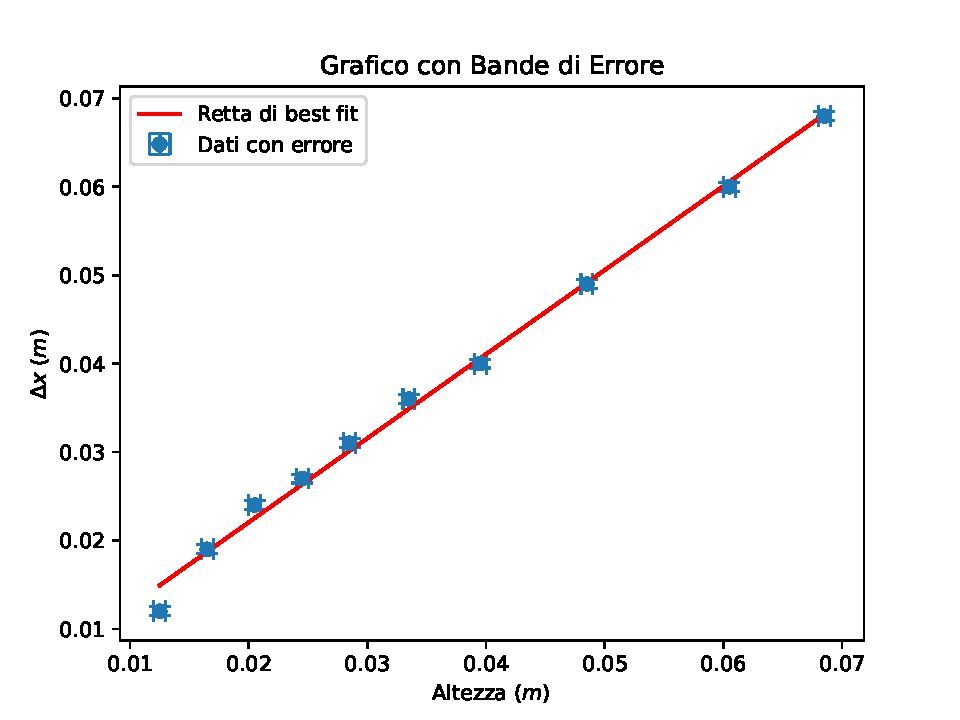
\includegraphics[width=0.75\textwidth]{./figures/grafico1}
	\caption{Il grafico mostra lo spostamento $x$ in funzione dell'altezza dell'acqua. I punti blu rappresentano le nostre misurazioni mentre in rosso è rappresentata la retta di best-fit calcolata utilizzando il metodo dei minimi quadrati (vedi Sezione (2.2)).\\
	Coefficiente angolare: $b=0.95\pm 0.07$\\
	Si noti, dalla Legge (1), che il coefficiente angolare è adimensionale.}
\end{figure} 

Ricordiamo, dalla Legge (1), che il coefficiente angolare della retta di best-fit in Figura (10) è uguale a $(\tan(\theta_i)-\tan(\theta_r))$. Avendo misurato $\theta_i$ e la relativa incertezza, e avendo calcolato, mediante metodi statistici, il coefficiente angolare della retta di regressione e la relativa incertezza, è possibile stimare l'angolo di rifrazione:
\begin{equation}
	\theta_r=\arctan(\tan(\theta_i)-b)=43.1^{\circ}
\end{equation}
e la relativa incertezza, dalla Legge (17) e ponendo $\vec{x_0} = (\tan(\theta_i),b)$:
\begin{align}
	\Delta \theta_r&=\left(\frac{1}{\tan^2(\theta_i)-2b\tan(\theta_i)+b^2+1}\right)\Delta \tan(\theta_i) - \left(\frac{1}{b^2-2b\tan(\theta_i)b+\tan^2(\theta_i)+1}\right)\Delta b= \\
    &=2.1^{\circ}
\end{align}



